
\section*{Combat}
\DefineNamedColor{named}{eclipsered}{rgb}{0.686,0.566,0.482}
\definecolor{tablecolor}{named}{eclipsered}


Each \textbf{combat turn} (also called \textbf{action turn}) takes \SI{3}{s}.
%
In a single combat turn all characters act based on their \textbf{initiative} (1D6 + Initiative), going from high to low.
%
The player can then perform exactly \textbf{one} of the below:

\begin{itemize}
    \itembox \num{1} complex and \num{1} quick action,
    \itembox \num{1} task action and \num{1} quick action,
    \itembox \num{3} quick actions.
\end{itemize}

Additionally, player may take any number of automatic actions per combat turn.

\bigskip

\subsection*{Basics and Movement}


\begin{eptable}{ l | X }
   \epheader{2}{Action Examples}
   Automatic & Talk, base perception (\modifier{-20}), defend, drop, moving, \textellipsis\\
   Quick & Activate, explain, normal perception, draw gun, go cover, \textellipsis\\
   Complex & Aim, attack (gun, melee), examine, reload, complex device, \textellipsis\\
   Task & Anything longer than \SI{2}{s} (\eg, hack, repair, heal ...)\\
\end{eptable}


\bigskip

\begin{eptable}{ l | l | X }
   \epheader{3}{Movement}
   Base Movement & Automatic & Moves base rate (\eg, \SI{4}{m})\\
   Full Movement & Automatic & Moves full rate (\eg, \SI{20}{m}), \modifier{-20} to actions.\\
   Rushing & Complex & Moves base + full (\eg, \SI{24}{m})$^\dagger$.\\
   Jumping & Quick & Running: \SI{6}{m}$^\dagger$.\\
   Standing Up & Quick & Movement rate halved afterwards.\\
   Non-Standard & Complex & Swimming, climbing, \textellipsis for base move.\\
   Zero Gravity & - & Half movement rate$^\dagger$. Jump any length.\\
   High Gravity & - & See rules$^\dagger$.\\
\end{eptable}


\begin{figure}
\begin{tikzpicture}

% NEW PICTURE
\node[anchor=south west, inner sep=0] (position) at (0,0) {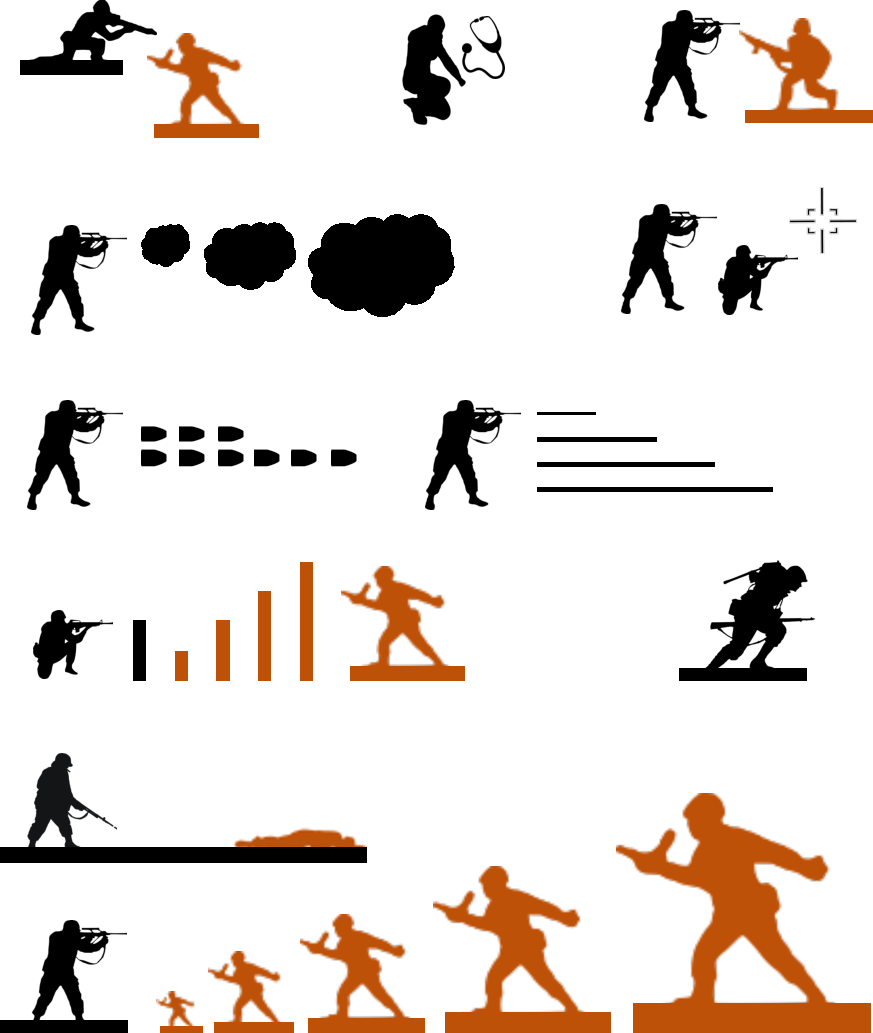
\includegraphics[width=1\columnwidth]{gfx/combat-diagram-combined}};
\begin{scope}[x={(position.south east)}, y={(position.north west)}]
    \node at (0.08,0.915) {+20};   % Superior position
    \node at (0.53,0.862) {-10 per WND / TRM};   % Wounded
    \node at (0.77,0.862) {-10 / -30};   % In melee
    \node at (0.182,0.725) {-10};   % vis min
    \node at (0.28,0.70) {-20};   % vis maj
    \node at (0.43,0.67) {-30 / 50\% miss};   % vis blind
    \node at (0.74,0.67) {+10};   % target short
    \node at (0.85,0.67) {+30};   % target long
    \node[anchor=south west] at (0.15,0.607) {+10 or +\dv{1d10} or 2 TGs};   % burst
    \node[anchor=south west] at (0.15,0.562) {+30 or +\dv{2d10} or 3 TGs};   % full auto
    \node[anchor=south west] at (0.15,0.52) {Suppressive Fire};   % full auto

    \node[anchor=south west] at (0.607,0.577) [align=left] {\scriptsize 2m};   % 2m
    \node[anchor=south west] at (0.607,0.55) [align=left] {\scriptsize 10m};   % 2m
    \node[anchor=south west] at (0.607,0.523) [align=left]{\scriptsize Range};   % 2m
    \node[anchor=south west] at (0.607,0.498)[align=left] {\scriptsize Range * n};   % 2m
    \node[anchor=south west] at (0.685,0.584) [align=left] {+10};   % 2m
    \node[anchor=south west] at (0.757,0.56) [align=left] { 0 };   % 2m
    \node[anchor=south west] at (0.822,0.537) [align=left]{ -10};   % 2m
    \node[anchor=south west] at (0.89,0.50)[align=left] { -n10\\-nd10 };   % 2m

    \node[anchor=south west] at (0.13,0.31) {-10};   % cover
    \node[anchor=south west] at (0.18,0.31) {-10};   % cover
    \node[anchor=south west] at (0.225,0.31) {-20};   % cover
    \node[anchor=south west] at (0.275,0.31) {-30};   % cover
    \node[anchor=south west] at (0.325,0.31) {50\%};   % cover

    \node[anchor=south west] at (0.82,0.31) {-20};   % running

    \node[anchor=south west] at (0.13,0.182) {-10};   % prone

    \node[anchor=south west] at (0.175,-0.03) {-30};   % size
    \node[anchor=south west] at (0.26,-0.03) {-10};   % size
    \node[anchor=south west] at (0.40,-0.03) {0};   % size
    \node[anchor=south west] at (0.57,-0.03) {+10};   % size
    \node[anchor=south west] at (0.82,-0.03) {+30};   % size

\end{scope}

\end{tikzpicture}
% This causes "Underfull \hbox" ...
% \caption{Common Ranged Attack Modifiers}
\end{figure}


\bigskip


The basic combat sequence:

\begin{itemize}
    \itembox \textbf{Declare Attack}. Skill depends on weapon type, \eg., Melee, Gun, Athletics (grenades), Interface (weapon system).
    \itembox \textbf{Declare Defense}. Melee (Melee, Fray), Ranged (Fray / 2). Psi (Willpower). Full Defense (\modifier{+30} bonus when used as complex action).
    \itembox \textbf{Apply Modifiers}. See Modifier tables.
    \itembox \textbf{Make Opposed Tests}. Both opponents roll.
    \itembox \textbf{Determine Result}. Handled as opposed test. Per attacker \textbf{superior success} inflict \dv{1d6} more. If \textbf{attacker critical} double damage.
    \itembox \textbf{Roll Damage}. Also apply any special damage weapon might cause.
    \itembox \textbf{Apply Armor}. Subtract remaining armor from damage. \textbf{Armor piercing} halves target armor.
    \itembox \textbf{Apply Damage}. Record damage. If accumulated damage exceeds Durability target incapacitated. If exceeds Death Rating target destroyed.
    \itembox \textbf{Determine Wounds}. Each multiple above Wound Threshold inflicts wound.
\end{itemize}


\begin{figure}[htbp!]%
   \centering
   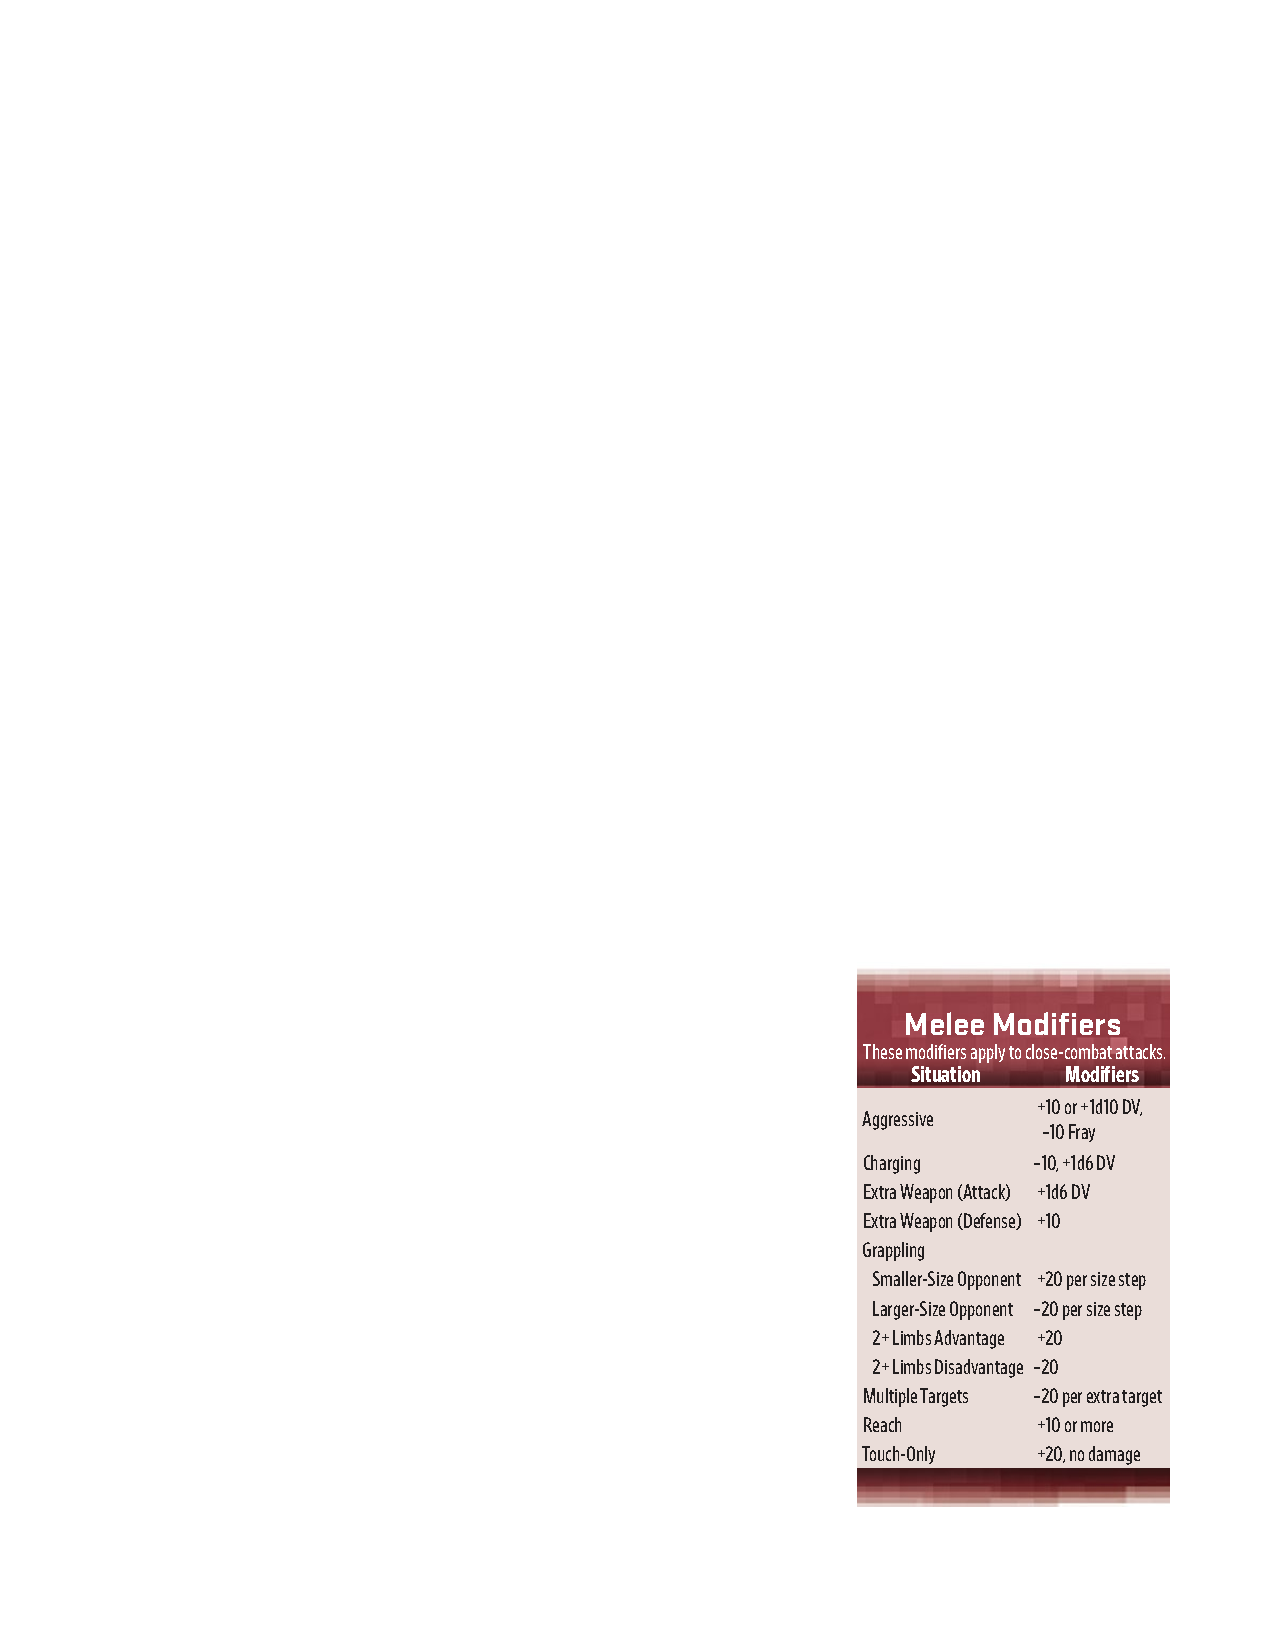
\includegraphics[scale=0.95]{gfx/combat-melee-modifiers}%
\end{figure}%

\begin{figure}[htbp!]%
   \centering
   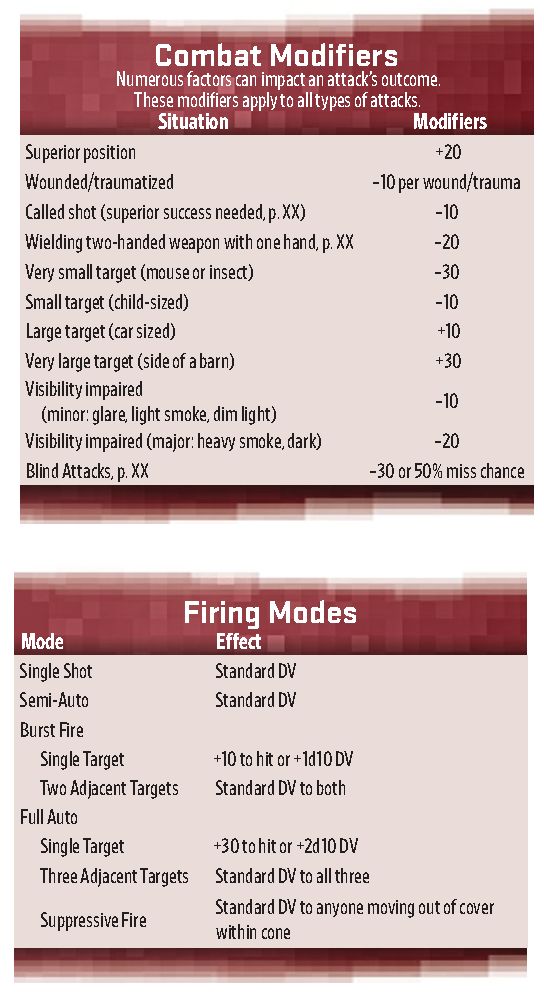
\includegraphics[scale=0.95]{gfx/combat-combined-fire-mod}%
\end{figure}%

\begin{figure}[htbp!]%
   \centering
   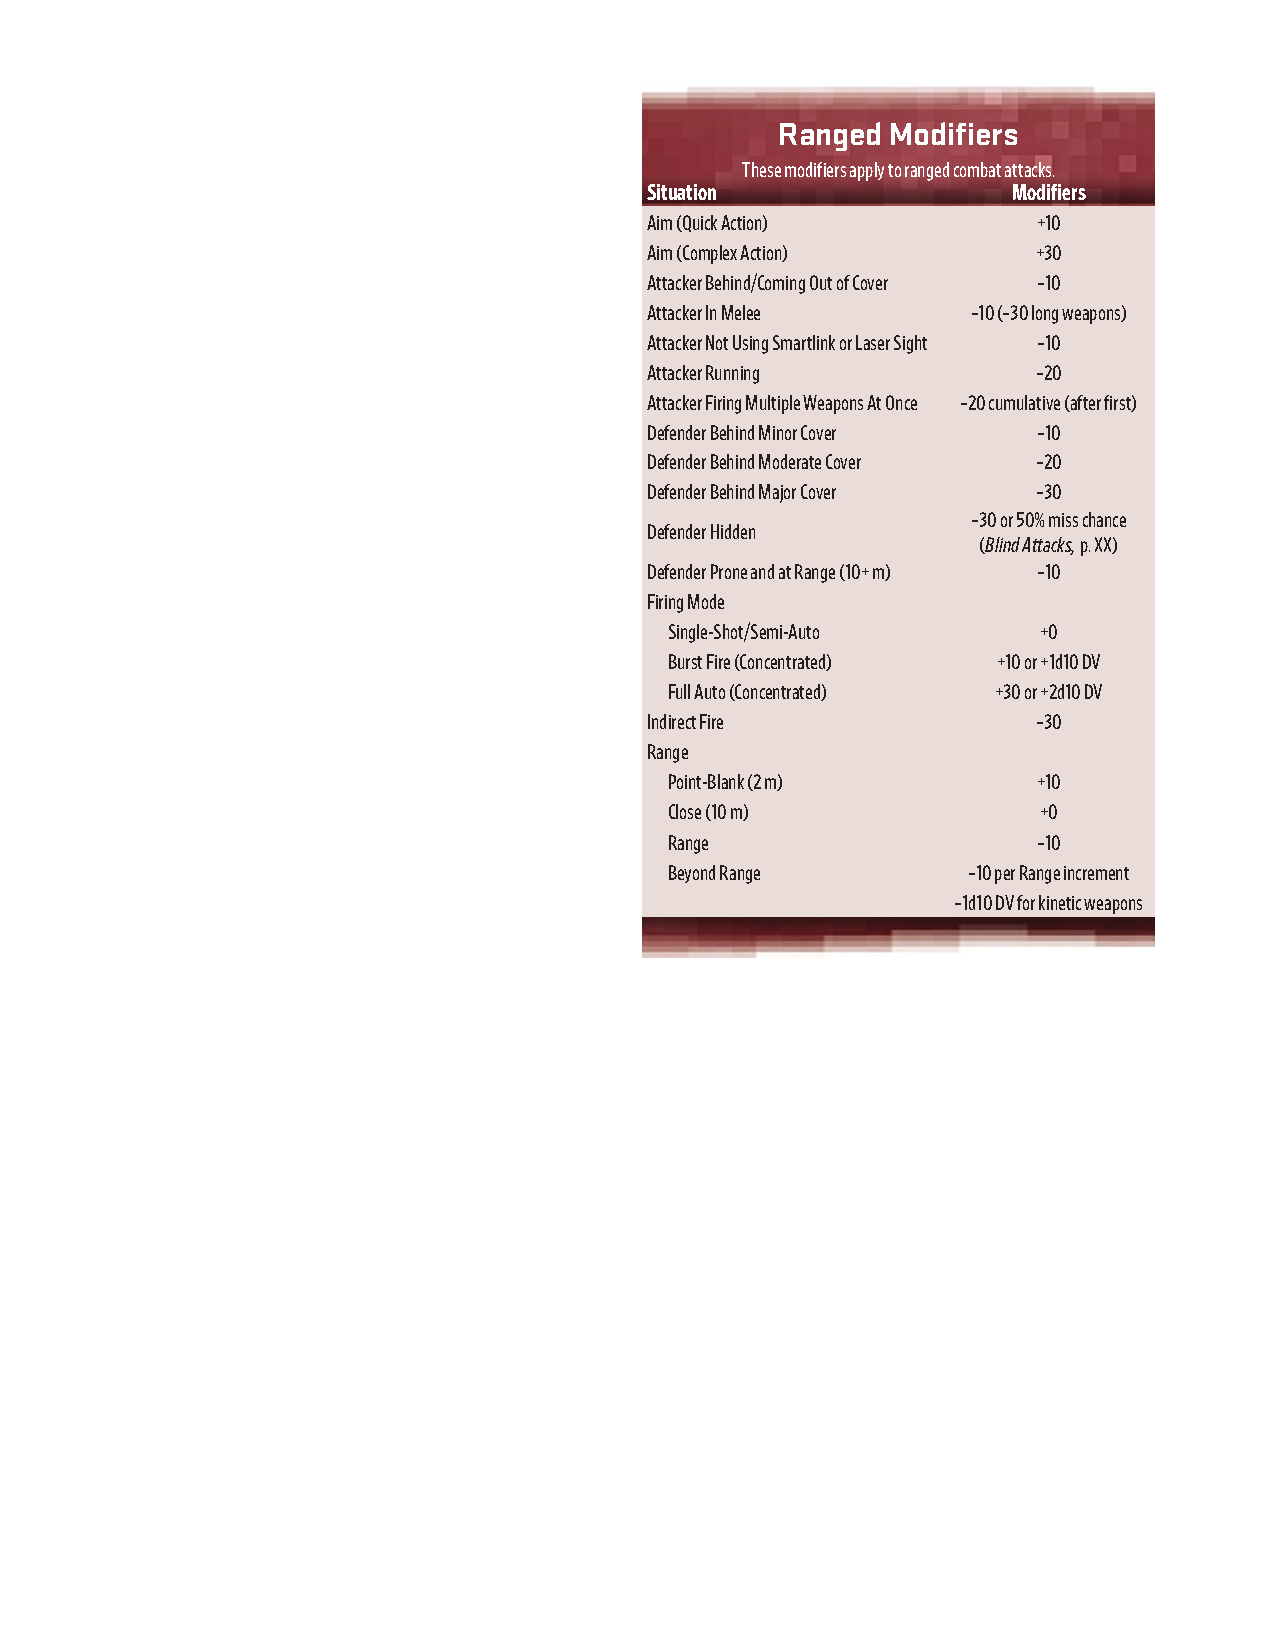
\includegraphics[scale=0.95]{gfx/combat-ranged-modifiers}%
\end{figure}%


\subsection*{Surprises}

\begin{itemize}
    \itembox Make opposed test between \skill{Infiltration} and \skill[-20]{Perception}.
\end{itemize}


\subsection*{Attacks}


\begin{eptable}{ l | X }
   \epheader{2}{Special Attacks}
   Area of Effect & Cone or Blast: DV/2 on successful Fray/2, unless near cover.\\
   Centered Blast & DV drops by \modifier{-2} for each meter from center.\\
   Uniform Blast & All in range full DV. Drops by \modifier{-2} for each meter outside.\\
   Cone & See Cone Attack table.\\
   Helpless Target & Roll attack. Success target dies. Fail max DV. OOC only.\\
   Called Shot & Attack with \modifier{-10}. On superior success see Called Shots table. \\
   Shock Attack & Only affects bio morphs, not synths. Details below. \\
   Social Attack & Opposed test \skill{Provoke} vs \skill{WIL}. See table Social Attacks. \\
   Sweeping Attack & With beam attack treat miss as aim +10 for next round. \\
   2+ Weapons & Each weapon separate attack, cumulative \modifier{-20} after first. \\
\end{eptable}

\begin{itemize}
    \itembox \textbf{Shock Attack}:
    Inflict shock without damage in melee: \skill[+20]{Melee}. Inflict shock plus
    damage requires is regular \skill{Melee}.
    \textbf{When hit} with shock effect make \skill{SOM} check, apply
    Energy Armor as positive modifier, if large \modifier{+30}, if small
    \modifier{-30}. \textbf{Failure}: lost neuromuscular control, fall, incap. for \num{1} turn (\modifier{+2} per sup. fail) and stunned
    for \SI{3}{min}. \textbf{Success}: stunned \num{3} turns.
    Synthmorphs are immune to shock, but mesh access disrupted for duration.
    General hardware might be disrupted.
    %
\end{itemize}

\bigskip

\begin{eptable}{ l | X }
   \epheader{2}{Cone Attack}
   Point Blank \& Close & Affects \num{1} target, \dv{+1d10}.\\
   Range & Affects \num{2} targets \SI{1}{m} of each other.\\
   Beyond Range & Affects \num{3} targets \SI{2}{m} of each other, \dv{-1d10}\\
\end{eptable}

Cone attack requires weapon that does cone damage.

\bigskip

\begin{eptable}{ l | X }
   \epheader{2}{Called Shot Results}
   Weak spot & Armor halved. GM might rule has no weak spot.\\
   Disarm & Victim gets half DV. Make \skill[-30]{SOM} or weapon off \dice{1d10} m$^\dagger$.\\
   Knockdown & Applies \textit{prone} condition. \\
   Redirect & Move opponent \SI{2}{m}. May make \skill[-30]{REF} to save. \\
   Special Target & Inflict other status conditions (\eg, blinded, hindered). \\
\end{eptable}


All Called Shots results \textit{only} apply if attacker succeeded
with \modifier{-10} attack \textit{AND} scores superior success.
Extra superior success can sometimes be used to increase modifiers or
inflict additional damage (e.g, full instead of half). See rule book for details.

\bigskip


\begin{eptable}{ l | X }
   \epheader{2}{Social Attacks}
   Calm & Soothe opponent into pausing hostilities temporarily.\\
   Fluster & Opponent \modifier{-10} for next action, additional \modifier{-10} per. sup. success.\\
   Inspire & NPC receives \modifier{+10} next action.\\
   Intimidate & Make opponent not attack, s.o. else, take cover, run away \num{1} turn.\\
   Taunt & Force opponent to attack you with their next action.\\
\end{eptable}

Also consult Social Modifiers table in the following chapter.

\bigskip

\subsection*{Objects \& Cover}


\begin{figure}[h!]%
   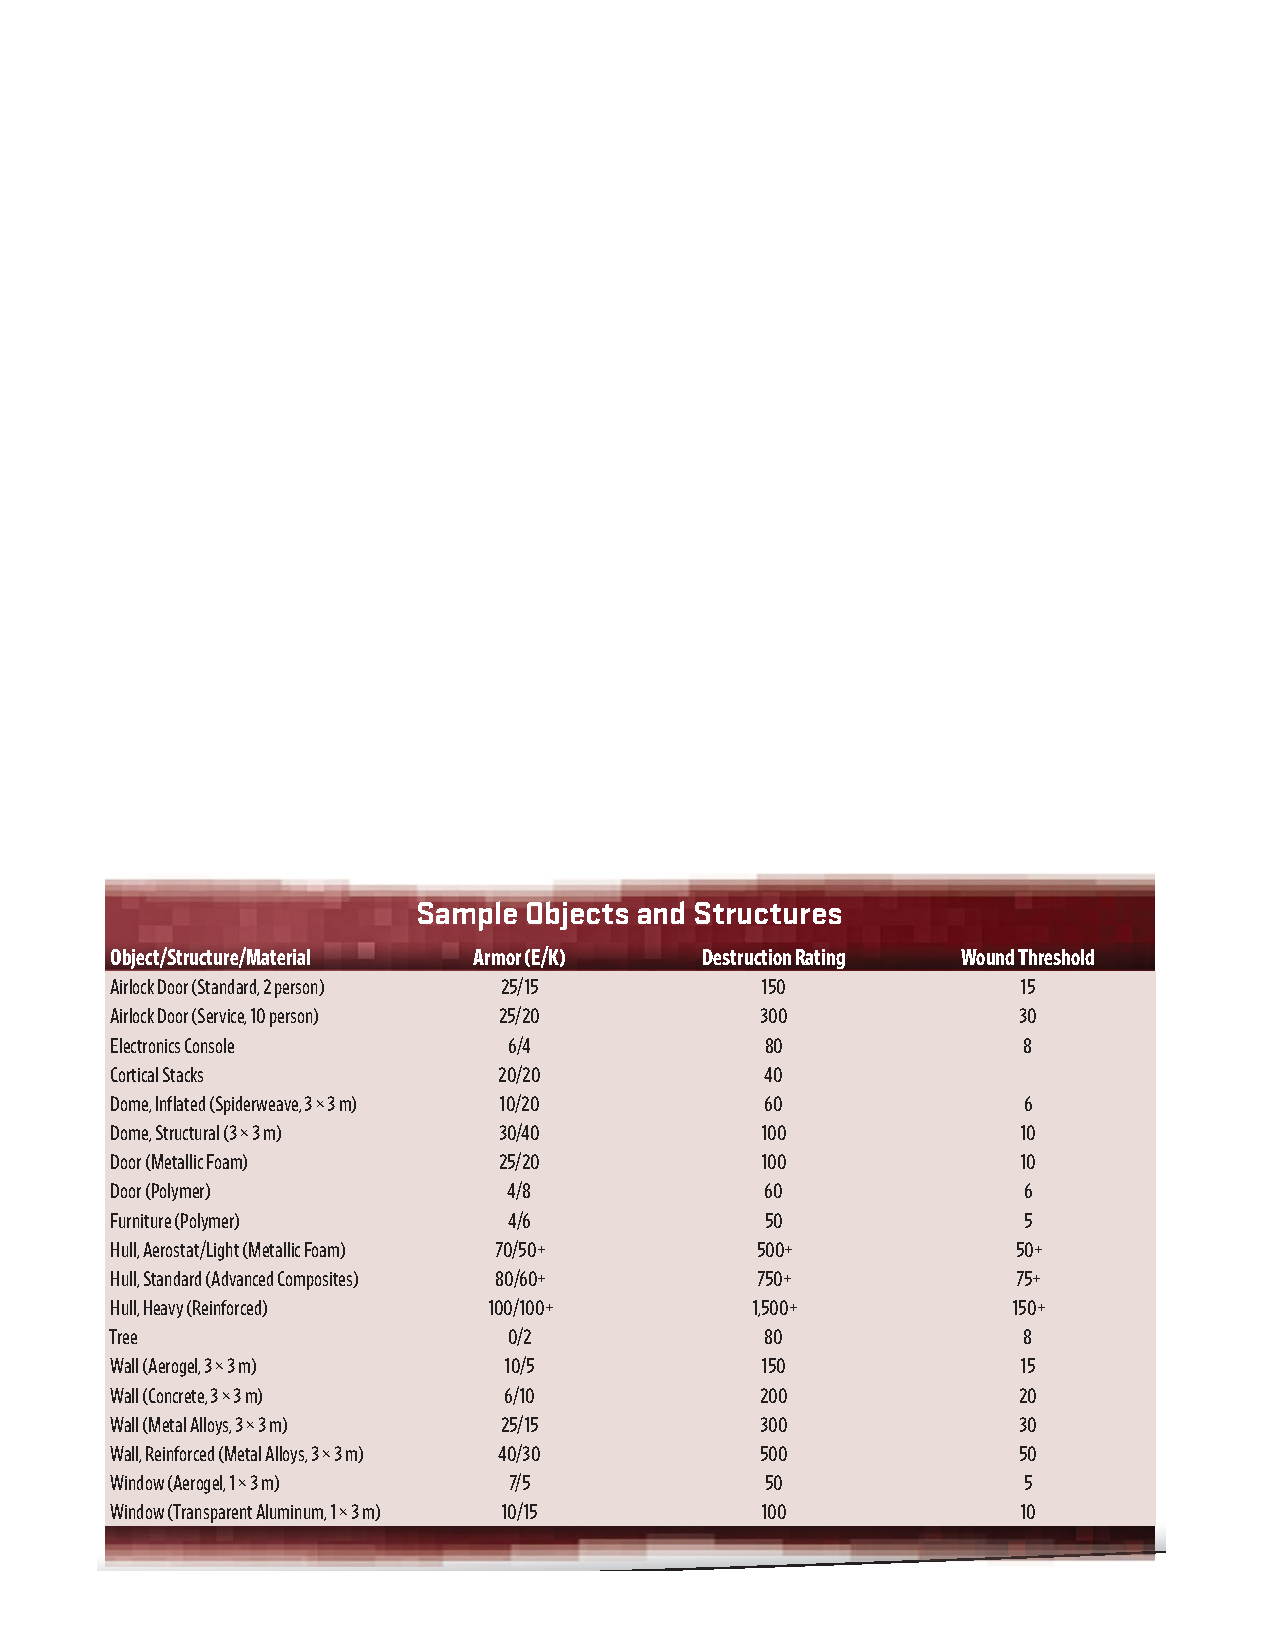
\includegraphics[scale=0.71]{gfx/combat-objects}%
\end{figure}%

\begin{eptable}{ X }
   \epheader{1}{Shooting Through Objects}
   Ranged kinetic attacks do only $1/2$ damage after armor subtracted.\\
   AoE kinetic, beam, energy attacks apply normal damage.\\
   Devices \modifier{-10} per wound, or stop working totally. \\
   Simple objects \SI{.5}{m} hole per wound.
\end{eptable}


\bigskip

\subsection*{Conditions}


\begin{eptable}{ l | X }
   \epheader{2}{Conditions}
   Blinded & All physical \modifier{-30}, still miss \SI{50}{\percent}. Skill check to move full.\\
   Confused & \skill[-30]{COG} p. turn. Failed: mutter; flee; rnd. attack or action.\\
   Dazed & No action except base move and defend.\\
   Deafened & Cannot hear. Initiative \modifier{-3}, Perception \modifier{-30}.\\
   Grappled & No action (even Fray) except Melee / SOM \modifier{-30} to escape.\\
   Incapacitated & No action whatsoever (not even defensive).\\
   Impaired & Suffer \modifier{-10}, \modifier{-20}, \modifier{-30}, depending on condition. \\
   % Paralyzed & No physical action (not even defensive). Mental / Mesh allowed. \\
   Prone & Quick action to get up. Melee opponent \modifier{+20}, ranged \modifier{-10}.\\
   Stunned & Suffer \modifier{-30} physical, \modifier{-10} mental.\\
   Unconscious & Helpless. Treat bios w. stim, cases w. \skill[-30]{INT} if DV < DUR.\\
\end{eptable}

Conditions can be set by weapons or circumstances.

\bigskip

\subsection*{Weapon and Gear Properties}

\begin{eptable}{ l | X }
   \epheader{2}{Weapon Traits}
   Armor Piercing & Inflicts \dv{-1d10}, but halves armor.\\
   Blinding & No anti-glare: \skill{REF} or blind \num{1} turn$^\dagger$. Perm. on crit.\\
   Concealable & Receive \modifier{30} for Infiltration hiding weapon.\\
   Entangling & Make \skill{REF} or be grappled. Superior attacks give \modifier{-10}.\\
   Fixed & Needs stand or be prone, otherwise \modifier{-20} to attack.\\
   Fragile & Item breaks or becomes unusable on superior fail.\\
   Knockdown & Target \skill{REF} or be knocked down.\\
   Lacks Smartlink & Receive \modifier{-10} to attack.\\
   Long & Give \modifier{-30} when firing in melee, no +10 on point blank.\\
   No Close & Cannot be used close or at point-blank.\\
   No Point-Blank & Cannot be used at point-blank.\\
   Pain & Target \skill{WIL} or flee \num{1} turn, \modifier{-20} to next action$^\dagger$.\\
   Paralyzing & Target \skill{REF} or paralyzed, \skill[-30]{REF} on sup. attack.\\
   Shock & Inflicts shock effect.\\
   Single Use & Can only be used once.\\
   Steady & Ignores range modifiers.\\
   Stun & Target \skill{SOM} or stunned$^\dagger$.\\
   Touch Only & Requires a touch to hit, +20, but no DV inflicted.\\
   Two-Handed & Needs two hands, or \modifier{-20} used with one.\\
\end{eptable}

See core book for details on traits for given weapon / ammunition.


\bigskip


\begin{eptable}{ l | X }
   \epheader{2}{Seekers \& Grenades}
   Adjust Blast Radius & Declare less (uniform) or reduction per meter (CAE).\\
   Jumping Grenades & \skill{REF} and \dv{+1d10} for you, but -(AV+10) others.\\
   Sticky & No scatter on hit.$^?$\\
   Throw Back & \skill{REF} to throw back if in range.\\
\end{eptable}

\begin{itemize}
   \itembox \textbf{Scatter}: On miss, roll 1 direction die (2D, gravity) or
   2 direction die (3D, microgravity) and distance die (as meters). Distance
   double per superior.
   %
\end{itemize}

\begin{figure}[h!]%
   \centering
   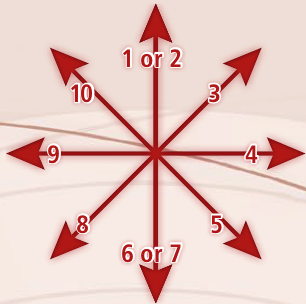
\includegraphics[scale=0.71]{gfx/combat-scatter}%
\end{figure}%




\bigskip

\begin{eptable}{ l | X }
   \epheader{2}{Trigger Conditions}
   Airburst & Explode after certain distance. Might ignore cover.\\
   Impact & Explode when hit. Resolve immediately.\\
   Proximity & Range up to \SI{3}{m}. Fixed \num{3} turn delay after activation.\\
   Signal & Explodes when transmitted signal over wireless.\\
   Timer & Minimum: end of next action turn.\\
\end{eptable}


\bigskip

\begin{eptable}{ X }
   \epheader{1}{Tactical Networks}
   Collate maps, tag spacial features.\\
   Share real time position information.\\
   Share sensory input between members.\\
   Encrypted communication.\\
   Smartlink / weapon data.\\
   Overwatch, \modifier{+10} against surprises.\\
   Indirect fire, help distant targets to aim.\\
   Analysis with real time suggestions and warning.\\
\end{eptable}
